\documentclass[10pt,a4paper]{article}

\usepackage[a4paper,margin=1.6cm,top=1.5cm,bottom=1.6cm]{geometry}
\usepackage[default]{sourcesanspro}
\usepackage{amsmath}
\usepackage{graphicx}
\usepackage[table]{xcolor}
\usepackage{enumitem}
\usepackage{booktabs}
\usepackage{caption}
\usepackage{subcaption}
\usepackage{float}
\usepackage{tikz}
\usetikzlibrary{arrows.meta}
\usepackage{titlesec}
\usepackage{microtype}
\usepackage[hidelinks]{hyperref}

\definecolor{ink}{HTML}{1C2B36}
\definecolor{accent}{HTML}{176783}
\definecolor{limit}{HTML}{C0392B}
% Layer-stack bands, bottom to top.
\definecolor{L0}{HTML}{8FA3B8}\definecolor{L1}{HTML}{C9A227}\definecolor{L2}{HTML}{4A6A96}\definecolor{L3}{HTML}{6B7785}
\definecolor{L4}{HTML}{7C8A4A}\definecolor{L5}{HTML}{DD7D2B}\definecolor{L6}{HTML}{C0392B}\definecolor{L7}{HTML}{2E8B57}
\hypersetup{colorlinks=true,urlcolor=accent,linkcolor=accent}

\graphicspath{{figures/}}
\setlength{\parindent}{0pt}
\setlength{\parskip}{4pt}
\setlist{nosep,leftmargin=12pt,topsep=2pt}
\captionsetup{font=small,labelfont={bf,color=accent},skip=3pt}
\captionsetup[sub]{font=footnotesize,skip=1pt}
\titleformat{\section}{\large\bfseries\color{ink}}{\thesection}{8pt}{}
\titleformat{\subsection}{\normalsize\bfseries\color{accent}}{\thesubsection}{6pt}{}
\titlespacing*{\section}{0pt}{8pt}{3pt}
\titlespacing*{\subsection}{0pt}{6pt}{2pt}

% One layer: screenshot on the left, what was added and how on the right.
\newcommand{\layer}[4]{%
  \noindent\begin{minipage}[t]{0.43\linewidth}\vspace{0pt}
    \includegraphics[width=\linewidth]{#1}
  \end{minipage}\hfill
  \begin{minipage}[t]{0.545\linewidth}\vspace{0pt}
    {\bfseries\color{accent}#2}\par\vspace{1pt}
    {\small #3\par}
    {\footnotesize\color{limit}#4}
  \end{minipage}\par\vspace{7pt}}

\begin{document}

\noindent\raisebox{-0.5\height}{
\includegraphics[height=0.95cm]{logo_dynacity}}\hfill
\raisebox{-0.5\height}{
\includegraphics[height=1.15cm]{logo_msfea}}\par\vspace{10pt}
{\color{ink}\LARGE\bfseries DynaCITY Web Simulator}\par\vspace{3pt}
{\color{accent}\large John Kofdarelli}\par\vspace{1pt}
{\small 3 November 2026}\par
\vspace{4pt}\textcolor{accent}{\rule{\linewidth}{0.6pt}}

The DynaCITY web simulator is a browser application that shows Beirut in 3D and lets a planner test changes to its streets. A Python server (FastAPI) loads the data and runs the traffic simulation. The browser draws a CARTO base map with MapLibre GL and stacks 3D layers on top with deck.gl. This note follows the order in which the layers were added. Each step lists the data set used and how it was integrated, followed by the SUMO traffic simulation and the pedestrian model. All screenshots come from the running application, and the six layer views share one camera, looking east across the Beirut River.

\section{Building the map, layer by layer}

Figure~\ref{fig:stack} shows the whole stack at once. Each layer sits on the ones below it and reuses their geometry. The six screenshots after it add the map layers one at a time, and Sections~2--4 cover the traffic and pedestrian layers.

% One band of the layer stack: level, colour, name, what it holds.
\newcommand{\band}[4]{%
  \pgfmathsetmacro{\yb}{#1*0.56}\pgfmathsetmacro{\yt}{\yb+0.47}\pgfmathsetmacro{\ym}{\yb+0.235}
  \pgfmathsetmacro{\wb}{3.05-0.06*#1}\pgfmathsetmacro{\wt}{\wb-0.22}
  \fill[#2] (-\wb,\yb) -- (\wb,\yb) -- (\wt,\yt) -- (-\wt,\yt) -- cycle;
  \node[white,font=\small\bfseries] at (0,\ym) {#3};
  \node[anchor=west,font=\footnotesize,text width=8.6cm,inner sep=0pt] at (3.35,\ym) {#4};}
\begin{figure}[H]
\centering
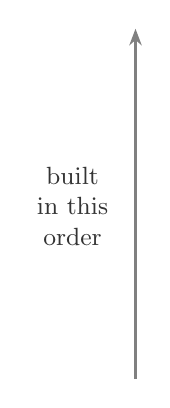
\begin{tikzpicture}
  \band{0}{L0}{Base map (CARTO)}{Vector tiles: land, water, street names}
  \band{1}{L1}{OpenStreetMap roads \& context}{10,818 road segments, lanes, 138 signals, crossings, parks, trees, paths}
  \band{2}{L2}{BBED buildings}{3,349 surveyed buildings with 2018 / 2022 / 2024 status}
  \band{3}{L3}{Beirut 001 3D model}{17,569 modelled buildings, ground grid and bridge decks}
  \band{4}{L4}{Overture surrounding buildings}{53,139 OSM and Microsoft footprints outside Beirut 001}
  \band{5}{L5}{Traffic data}{Tari'ak hourly speeds and CDR peak counts on every road}
  \band{6}{L6}{SUMO traffic simulation}{Simulated cars, closures, crashes and rerouting}
  \band{7}{L7}{Pedestrians \& street planner}{UNA walking flows, walkers, car-free streets, wider pavements}
  \draw[-{Stealth[length=6pt]},thick,gray] (-3.5,0) -- (-3.5,4.45);
  \node[align=center,font=\small,gray!40!black] at (-4.3,2.2) {built\\in this\\order};
\end{tikzpicture}
\caption{The layer stack of the web simulator, bottom to top.}\label{fig:stack}
\end{figure}

\layer{l1_basemap}{1 · Empty base map (CARTO)}{%
\begin{itemize}
\item \textbf{Data:} CARTO Voyager vector style and tiles, built on OpenStreetMap.
\item \textbf{Integration:} MapLibre GL draws the map, and deck.gl is attached as an overlay so every later layer shares its camera.
\item The style's open sea is repainted as water, and its flat building fills are faded so that 3D buildings can replace them.
\end{itemize}}{}

\layer{l2_roads}{2 · Road network (OpenStreetMap)}{%
\begin{itemize}
\item \textbf{Data:} drivable OSM ways fetched from the Overpass API, plus 30 OSM bus and van routes.
\item \textbf{Integration:} ways are split at shared nodes into a directed graph of 10,818 road segments (EPSG:32636). Each segment keeps its OSM class, lanes, one-way flag, and bridge or tunnel level. The graph also holds 138 OSM traffic signals, 26 turn bans and 253 mapped crossings.
\item Carriageways are drawn as lanes $\times$ 3.2\,m, with pavements and lane markings, and bridges are raised onto decks and piers.
\end{itemize}}{}

\layer{l3_landscape}{3 · Mapped landscape (OpenStreetMap context)}{%
\begin{itemize}
\item \textbf{Data:} a second Overpass extract over the same extent, fetched in five groups: landscape, mobility, places, buildings and infrastructure.
\item \textbf{Integration:} objects are merged by OSM type and ID, and every object keeps its tags and timestamp. The page draws ground surfaces (parks, plazas, sand, water channels), trees, footpaths and stairs. It currently holds about 1,500 tree features, 1,870 surfaces and 1,400 paths.
\end{itemize}}{}

\layer{l4_bbed}{4 · BBED buildings (Beirut Urban Lab, AUB)}{%
\begin{itemize}
\item \textbf{Data:} the Beirut Built Environment Database (BBED), 2024 layer: 3,349 surveyed buildings with use, floors, height and status in 2018, 2022 and 2024.
\item \textbf{Integration:} only an allowlist of fields is fetched from the ArcGIS service (no names or owner data). Raw status labels map to 8 canonical states (e.g.\ stable, under construction, vacant, demolished). Buildings are extruded to their recorded height and coloured by status. BBED drives the forecasting model, and ODbL attribution is kept.
\end{itemize}}{}

\layer{l5_beirut001}{5 · Beirut 001 3D city model}{%
\begin{itemize}
\item \textbf{Data:} Beirut 001 (Salim al-Kadi and team, January 2020), a 730\,MB Rhino model of the 12 municipal areas.
\item \textbf{Integration:} the model is read once and packed into a 7\,MB file. Each of its 17,575 solids is reduced to an outline, roof level and ground level, and 99.6\% of them are simple extrusions. It also keeps a 10\,m ground grid and the bridge meshes, which give 46 of 135 road bridges their measured deck heights.
\item \textbf{Placement:} the model has no coordinates. It is aligned to BBED by matching building-centre patterns (rotate, cross-correlate, then refine on nearest pairs): a $+1.344^\circ$ turn and a fixed shift. 687 buildings are provisionally linked to a BBED record, and the rest keep the model's own data.
\end{itemize}}{}

\layer{l6_overture}{6 · Surrounding buildings (Overture Maps)}{%
\begin{itemize}
\item \textbf{Data:} Overture Maps buildings (release 2026-09): OSM outlines plus Microsoft machine-learned footprints, 68,719 candidates.
\item \textbf{Integration:} Beirut 001 stays authoritative. Any footprint overlapping a Beirut 001 building by 10\% or more is dropped (15,193), never merged. This fills Bourj Hammoud, east of the river, and the suburbs.
\item \textbf{Heights:} only 159 footprints have a mapped height. The others take the median Beirut 001 height for the same footprint size (8.5\,m under 100\,m$^2$, 17\,m for 100--200\,m$^2$, about 25\,m for 200--800\,m$^2$).
\end{itemize}}{}

\section{Traffic and pedestrian models}

\subsection{Historical speeds and volumes}
\begin{itemize}
\item \textbf{Tari'ak Lebanon traffic data set:} about six million crowd-sourced vehicle speeds, 2014--2019, map-matched to OSM ways. Each road gets a median speed for every hour of the day. 5,812 segments with too few readings borrow their road class's hourly profile and are flagged as estimated.
\item \textbf{CDR Bus Rapid Transit study (2016--17):} AM and PM peak-hour vehicle counts on named Beirut roads. They are matched to OSM ways by name, summarised per road class, spread over the day with the probe readings' hourly shape, and scaled by lane count.
\end{itemize}

\subsection{SUMO microsimulation}
Every car on the map is a vehicle in \href{https://eclipse.dev/sumo/}{SUMO} (Eclipse SUMO 1.22), the open-source traffic simulator, which the server drives step by step through its TraCI interface.
\begin{enumerate}[leftmargin=14pt]
\item \textbf{Network:} the OSM road graph is exported to SUMO with the same 3.2\,m lanes, signals, turn bans and bridge levels. Each road's speed limit is the fastest of its Tari'ak hourly medians, i.e.\ its free-flow speed.
\item \textbf{Starting fleet:} cars per road = directional flow $\times$ road length $\div$ that hour's typical speed, using the CDR counts.
\item \textbf{Ongoing demand:} cars keep entering at the map edge (about 1,300 a minute at 08:00 and 1,600 at 17:00), and trips also start inside the city (about 2,200 and 2,800 a minute). Destinations are drawn at least 1\,km away in a straight line, which gives trips of about 4\,km.
\item \textbf{Routing:} shortest legal path (Dijkstra) over SUMO's lane connections, so turn bans hold. SUMO then handles car-following, lane changes, junction priority and signals at a one-second step.
\item \textbf{Check:} once the run has warmed up, the simulated speed on each road is compared with the Tari'ak median for that hour.
\item \textbf{Drawing:} the server sends only the cars in and around the camera view. The browser interpolates the one-second positions and draws 3D cars with paint variations, brake lights, indicators and night headlights.
\end{enumerate}

\subsection{Pedestrian flow model}
Pedestrian volumes follow \href{https://hdl.handle.net/1721.1/156355}{Sevtsuk et al.\ (2024), \emph{Pedestrian-oriented development in Beirut}, Cities 149} (\href{https://doi.org/10.1016/j.cities.2024.104927}{doi:10.1016/j.cities.2024.104927}). They are computed with MIT City Form Lab's open-source \href{https://github.com/City-Form-Lab/urban_network_analysis}{Urban Network Analysis (UNA)} tool.
\begin{itemize}
\item \textbf{Formula} (the paper's Table~2, weekday PM peak, 16:30--17:30):
\[\text{pedestrians/h} = 61.62 + 3.49\,F_{\text{amen}\to\text{amen}} + 0.08\,F_{\text{jobs}\to\text{homes}} + 0.08\,F_{\text{parks}\to\text{amen}} + 0.02\,F_{\text{homes}\to\text{worship}} + 9.77\]
Each $F$ is a gravity-based trip flow over the walking network, with an 800\,m radius and decay $\beta=0.002$.
\item \textbf{Inputs:} 11,890 OSM walkable segments (motorways and trunk roads excluded); 2,504 shops and services, 152 places of worship, 90 parks and 139 bus stops from OSM. Homes come from 17,308 Beirut 001 buildings (footprint $\times$ floors $\div$ 100\,m$^2$ per resident, about 460,000 people). Jobs use a proxy built from OSM offices, shops, schools and hospitals.
\item \textbf{Walkers on the map:} after the constant is removed (so quiet streets stay quiet), each segment's flow becomes people present ($\text{people/h} \div 3600 \times \text{length} \div 1.3\,\text{m/s}$). That gives 2,307 pavement segments and about 730 people citywide at any moment, each drawn as a small figure walking along the middle of the pavement.
\item \textbf{Check:} Hamra Street comes out busiest (up to about 370 per hour). Gouraud Street gives 158--267 per hour against the paper's published 173 at Gouraud $\times$ George Haddad.
\end{itemize}

\section{Traffic simulation in detail}
\begin{figure}[H]
\centering
\begin{subfigure}[t]{0.495\linewidth}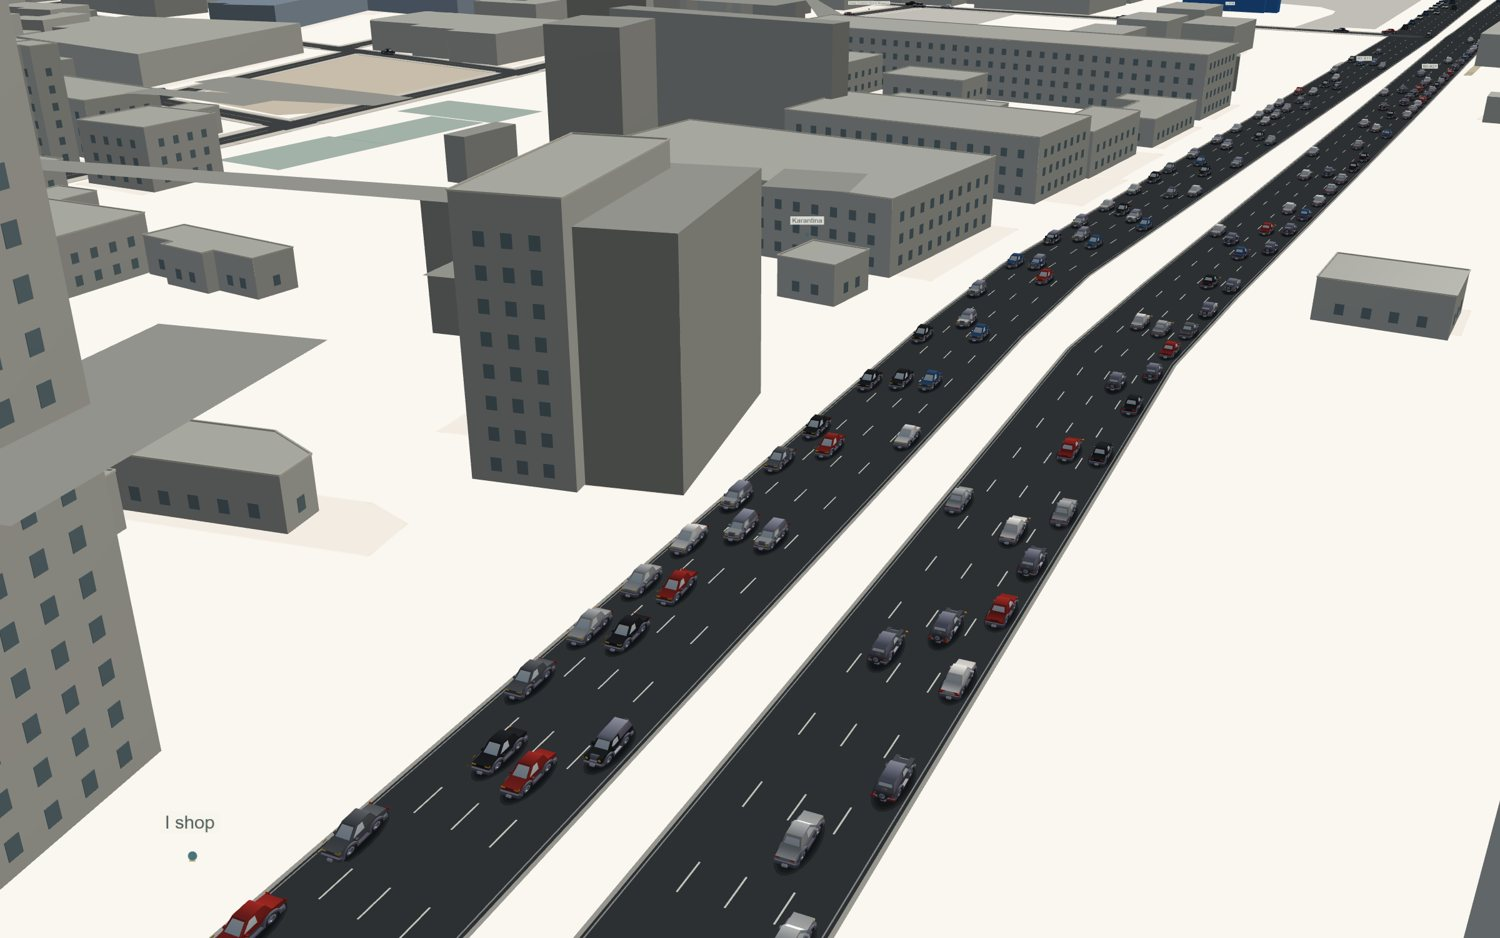
\includegraphics[width=\linewidth]{t_cars_helou}\caption{Charles Helou Highway, 08:00: every car is a SUMO vehicle.}\end{subfigure}\hfill
\begin{subfigure}[t]{0.495\linewidth}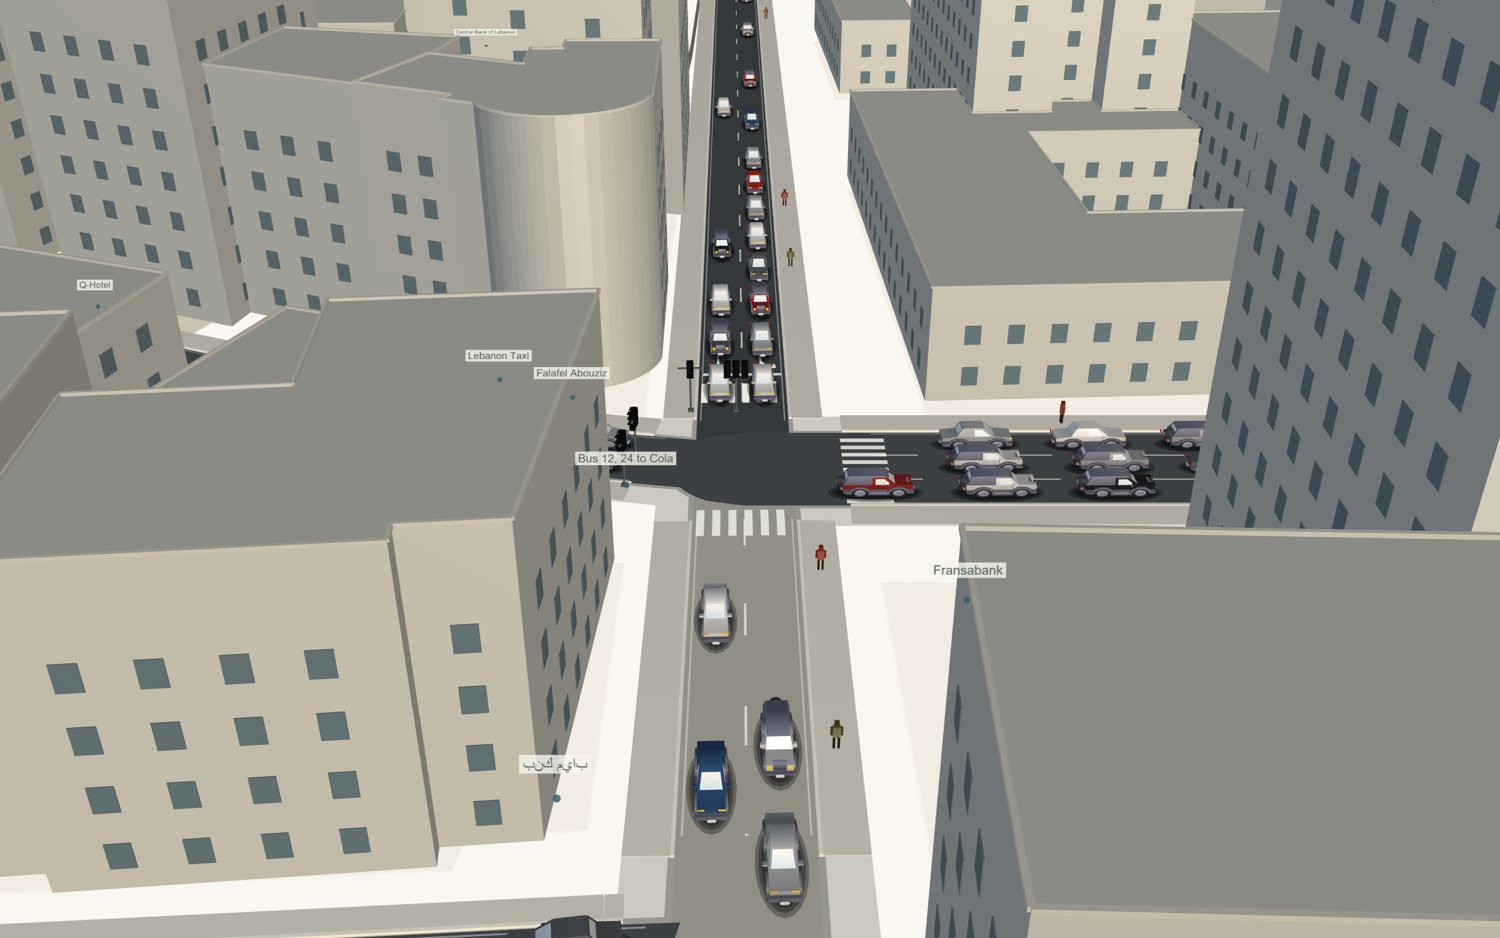
\includegraphics[width=\linewidth]{t_junction}\caption{Hamra, 17:00: cars queued at a red light, a zebra crossing and pavement walkers.}\end{subfigure}
\caption{Street-level view of the running simulation.}
\end{figure}

\textbf{Controls available in the Traffic panel} (Figure~\ref{fig:ui}):
\begin{itemize}
\item \textbf{Hour slider (00:00--23:00):} restarts SUMO with that hour's speeds, volumes and trip rates.
\item \textbf{Street view / Traffic colours:} asphalt, lane markings and crossings, or each road coloured by its historical speed relative to free flow (blue = near free flow, amber = slow, red = crawling).
\item \textbf{Simulated traffic lights:} red, amber and green come from SUMO's signal controllers. Up close they become 3D poles with turn arrows.
\item \textbf{Road events:} \emph{Make car-free} (close a segment) or \emph{Crash} (block it at a clicked point), on any number of segments.
\item \textbf{Comparison:} \emph{normal traffic vs your changes}, with live counts of rerouted, stopped and delayed vehicles.
\item \textbf{Optional settings:} incoming traffic from 0 to 2$\times$, pedestrian demand from 0 to 3$\times$, OSM bus and van routes, pause and reset.
\end{itemize}

\begin{figure}[H]
\centering
\begin{subfigure}[t]{0.328\linewidth}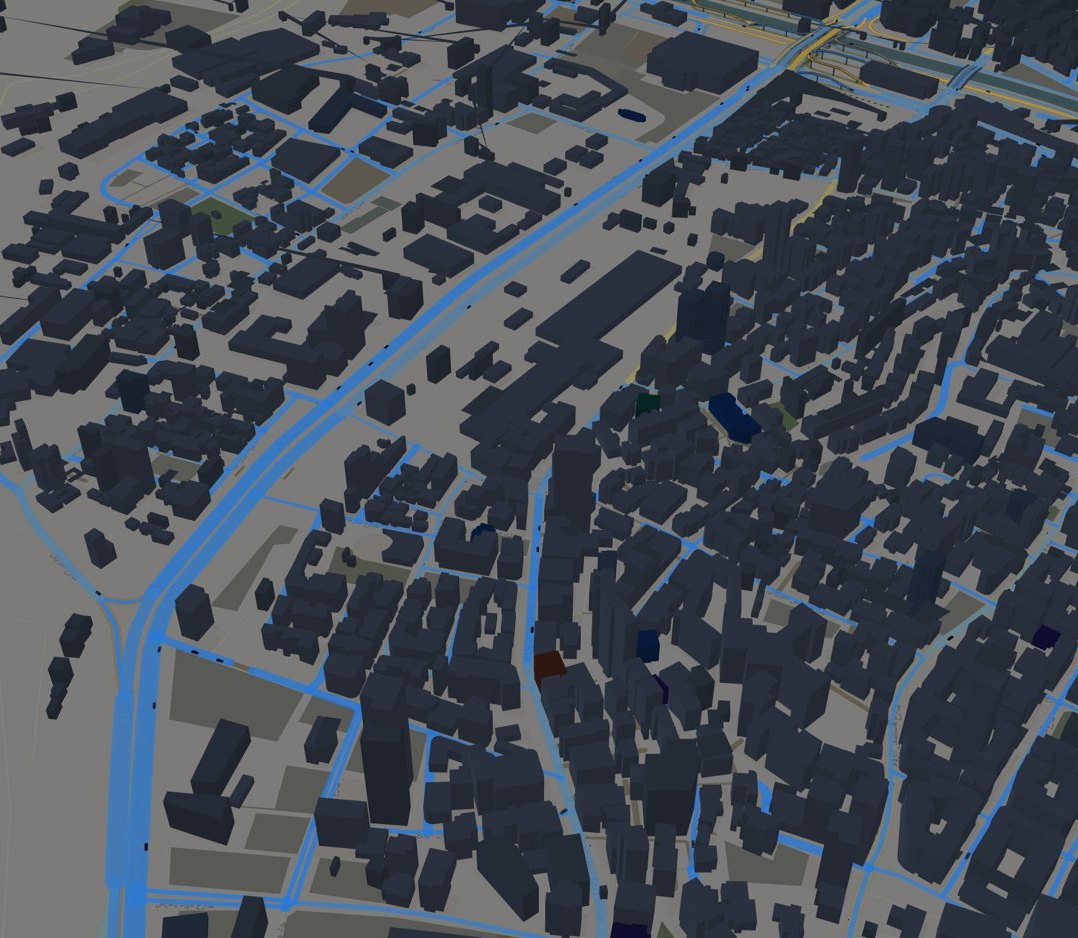
\includegraphics[width=\linewidth]{t_hour03}\caption{03:00: few cars, near free flow (night mode).}\end{subfigure}\hfill
\begin{subfigure}[t]{0.328\linewidth}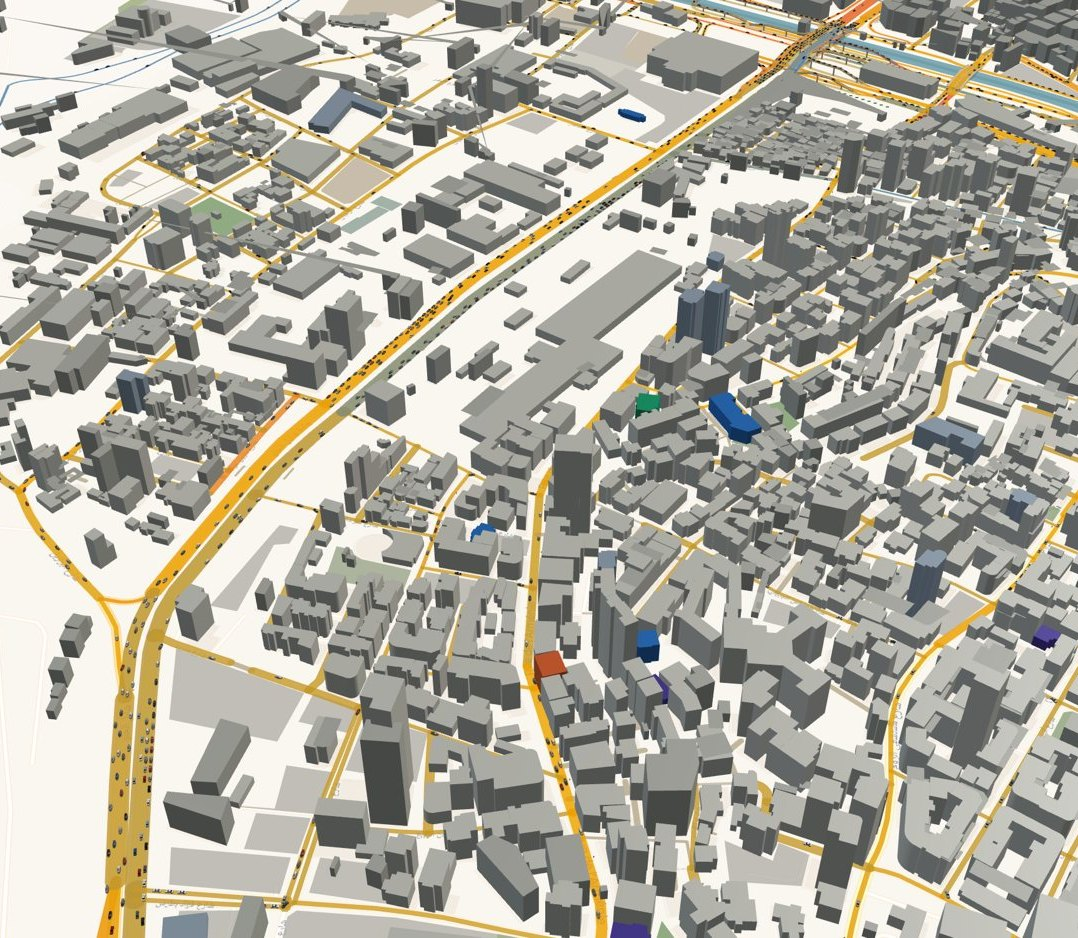
\includegraphics[width=\linewidth]{t_hour08}\caption{08:00: morning peak, slow (amber) arterials.}\end{subfigure}\hfill
\begin{subfigure}[t]{0.328\linewidth}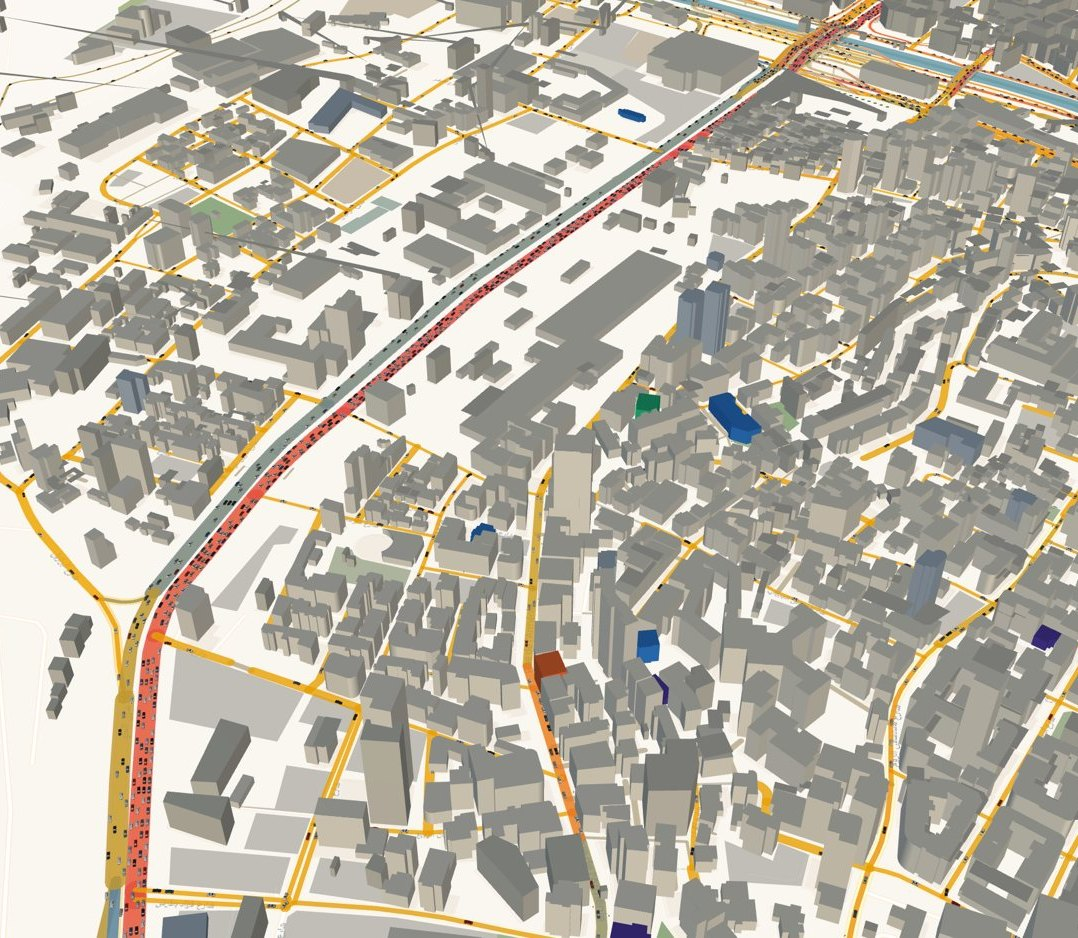
\includegraphics[width=\linewidth]{t_hour17}\caption{17:00: evening peak, Charles Helou crawling (red).}\end{subfigure}
\caption{Time of day, same view in Traffic colours. Colours are Tari'ak hourly medians. The number of cars and their trip rates change with the hour.}
\end{figure}

\subsection{Closing a road: how cars find a detour}
\begin{enumerate}[leftmargin=14pt]
\item \textbf{Fork:} just before the first change, the simulation is copied exactly (vehicles, signals and random-number state). One copy keeps the original roads and serves as the baseline. Both copies then run side by side with identical demand.
\item \textbf{Close:} in the scenario copy, the segment's lanes no longer allow cars, in both directions.
\item \textbf{Reroute:} every car whose remaining route uses the closed segment gets a new shortest legal route to the \emph{same} destination. Cars with no legal detour wait in a queue. Cars are never deleted or moved to another road.
\item \textbf{Measure:} the panel counts rerouted cars, cars without a detour, cars stopped inside the closure, overdue trips, and the delay of trips completed in both runs. Purple marks each road by how many rerouted cars it currently carries.
\item A \textbf{crash} works the same way but blocks the segment from the clicked point, and its marker sits where it was placed (Figure~\ref{fig:ui}b).
\end{enumerate}

\noindent\begin{minipage}[c]{0.6\linewidth}\centering
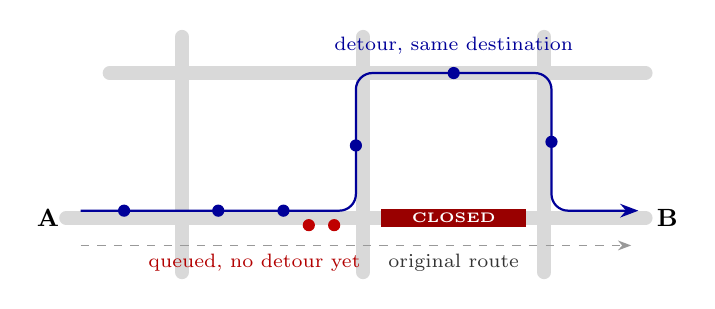
\begin{tikzpicture}[x=0.92cm,y=0.92cm,road/.style={line width=5pt,gray!30,line cap=round}]
  \draw[road] (0,0) -- (8,0); \draw[road] (0.6,2) -- (8,2);
  \foreach \x in {1.6,4.1,6.6} \draw[road] (\x,-0.75) -- (\x,2.5);
  \fill[red!60!black] (4.35,-0.12) rectangle (6.35,0.12);
  \node[white,font=\tiny\bfseries] at (5.35,0) {CLOSED};
  \draw[dashed,gray!80,-{Stealth}] (0.2,-0.38) -- (7.8,-0.38);
  \node[gray!40!black,font=\scriptsize] at (5.35,-0.62) {original route};
  \draw[blue!60!black,thick,-{Stealth},rounded corners=6pt] (0.2,0.1) -- (4.0,0.1) -- (4.0,2.0) -- (6.7,2.0) -- (6.7,0.1) -- (7.9,0.1);
  \foreach \p in {(0.8,0.1),(2.1,0.1),(3.0,0.1),(4.0,1.0),(5.35,2.0),(6.7,1.05)} \fill[blue!60!black] \p circle (2.2pt);
  \foreach \p in {(3.35,-0.1),(3.7,-0.1)} \fill[red!75!black] \p circle (2.2pt);
  \node[red!70!black,font=\scriptsize] at (2.6,-0.62) {queued, no detour yet};
  \node[blue!60!black,font=\scriptsize] at (5.35,2.38) {detour, same destination};
  \node[font=\small\bfseries] at (-0.25,0) {A}; \node[font=\small\bfseries] at (8.3,0) {B};
\end{tikzpicture}
\end{minipage}\hfill
\begin{minipage}[c]{0.37\linewidth}
\captionof{figure}{What SUMO does when a road closes. Cars heading for B turn off before the closure and take the fastest open path to the same destination. Cars that cannot turn yet wait in a queue and stay counted; none are deleted or moved. (Diagram.)}\label{fig:detour}
\end{minipage}
\vspace{6pt}

\begin{figure}[H]
\centering
\begin{subfigure}[t]{0.328\linewidth}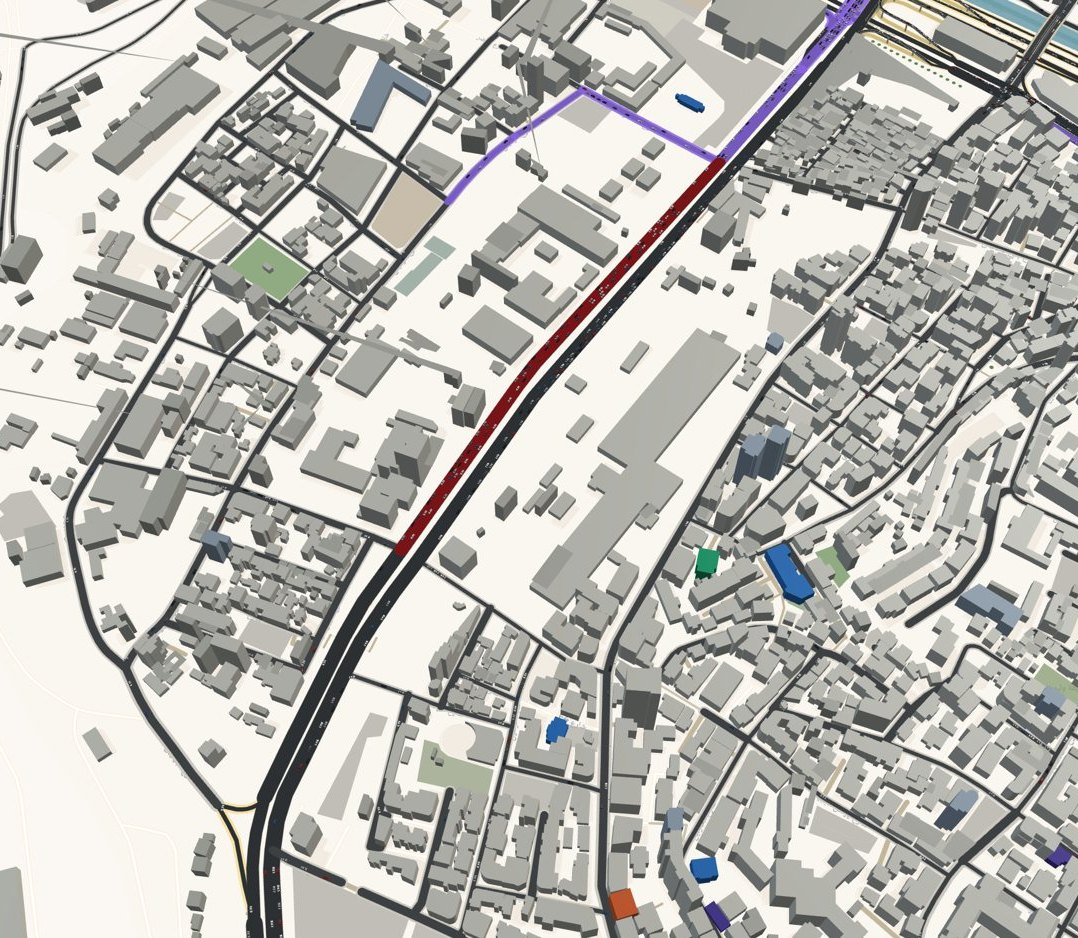
\includegraphics[width=\linewidth]{t_closure_overview}\caption{A 554\,m section of Charles Helou made car-free (red).}\end{subfigure}\hfill
\begin{subfigure}[t]{0.328\linewidth}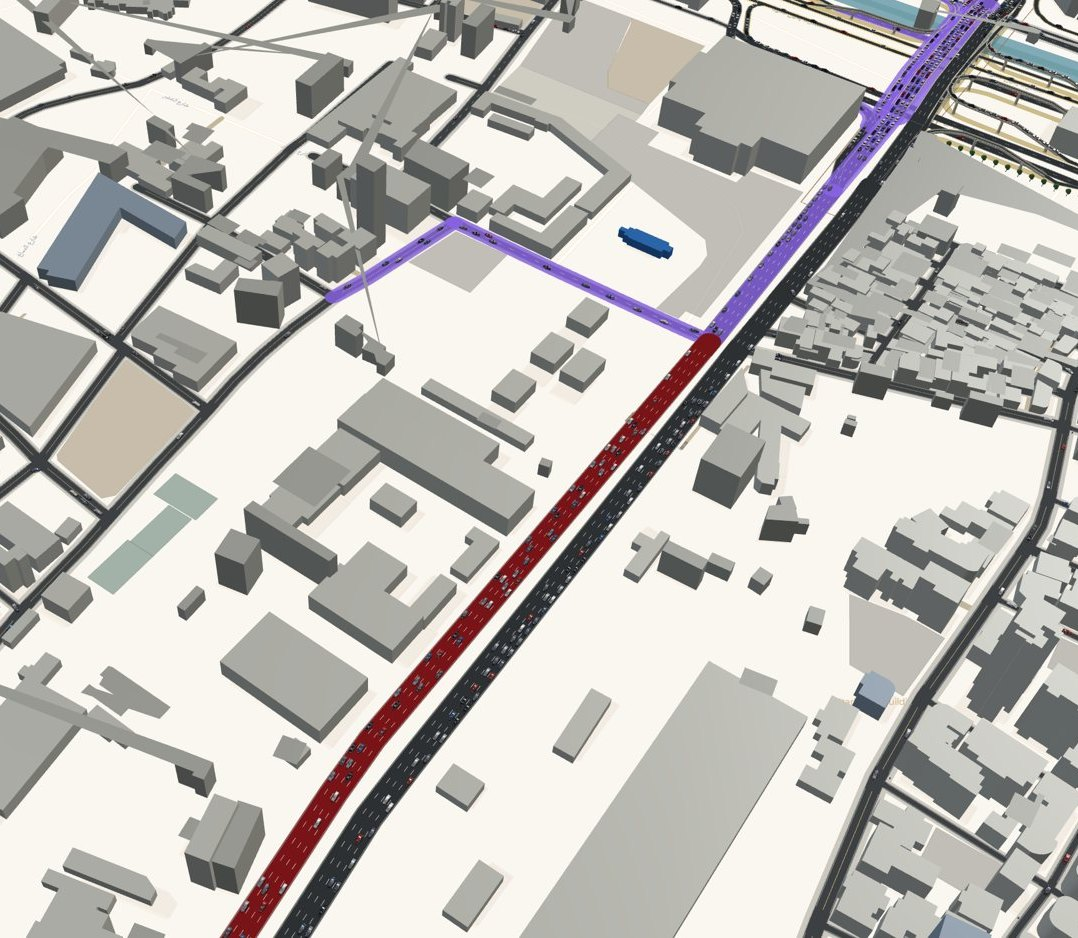
\includegraphics[width=\linewidth]{t_closure_east}\caption{Purple: roads where rerouted cars now drive.}\end{subfigure}\hfill
\begin{subfigure}[t]{0.328\linewidth}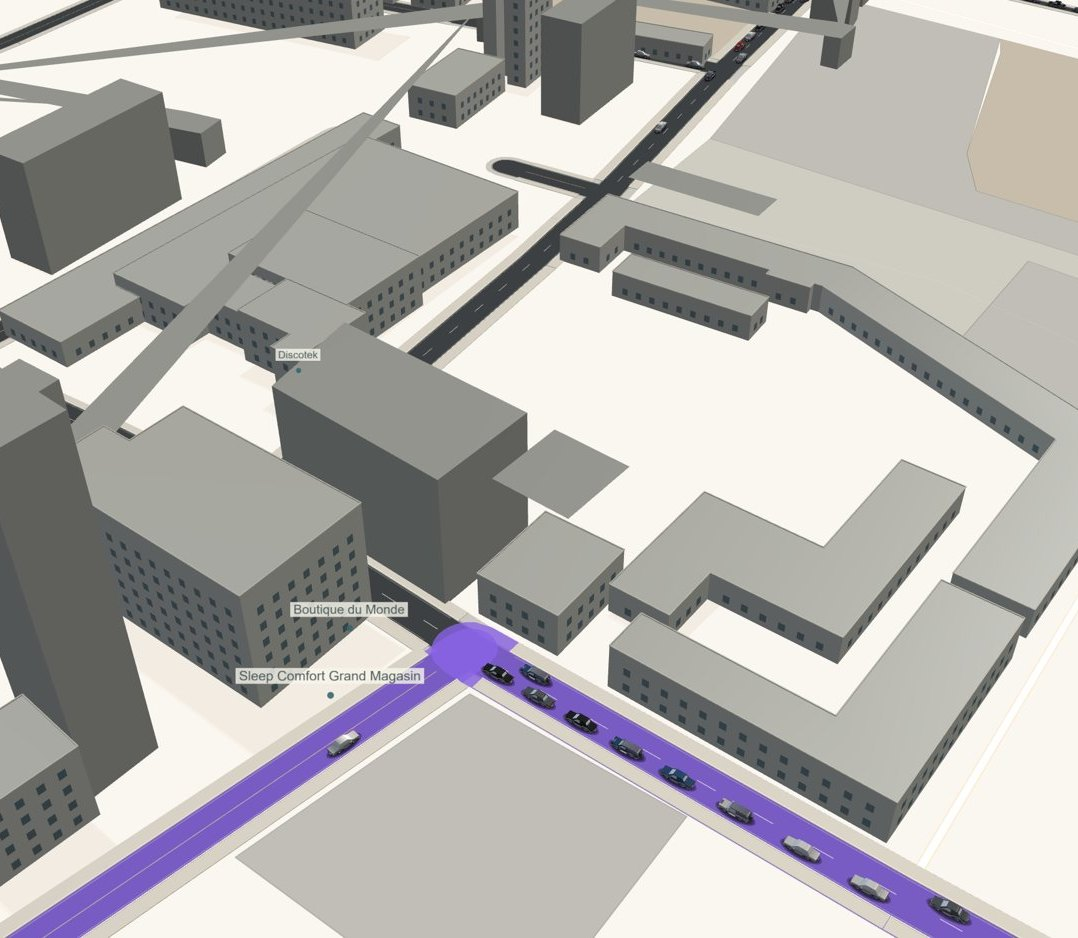
\includegraphics[width=\linewidth]{t_reroute_near}\caption{Close-up: rerouted cars on a side street.}\end{subfigure}
\caption{Closure of Charles Helou Highway at 08:00.}
\end{figure}

\begin{figure}[H]
\centering
\begin{subfigure}[t]{0.6\linewidth}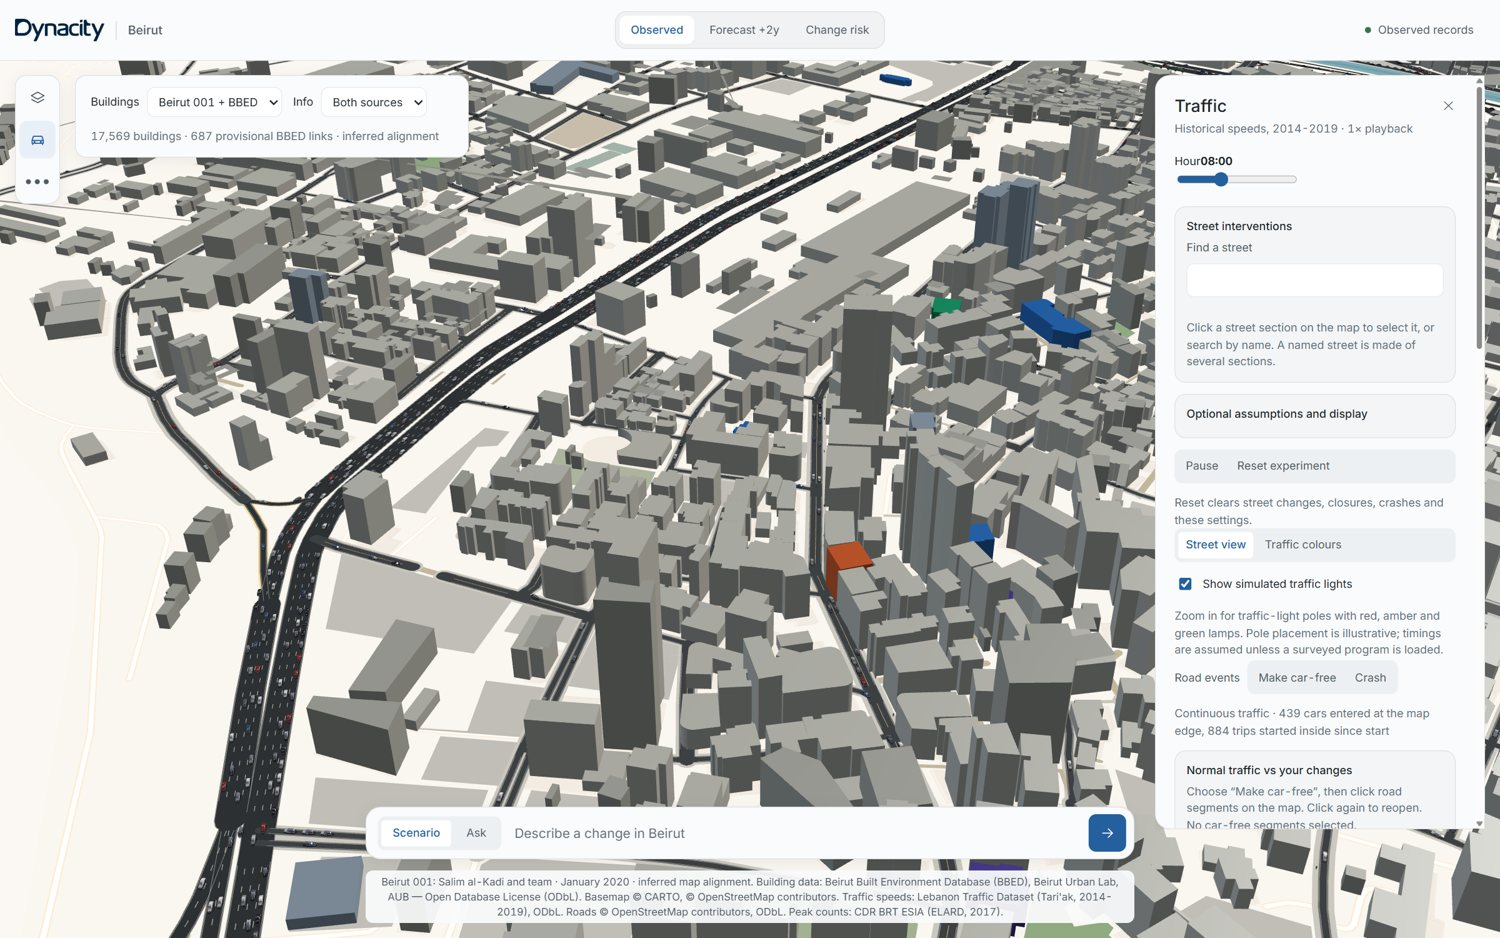
\includegraphics[width=\linewidth]{ui_overview}\caption{The interface with the Traffic panel open.}\end{subfigure}\hfill
\begin{subfigure}[t]{0.385\linewidth}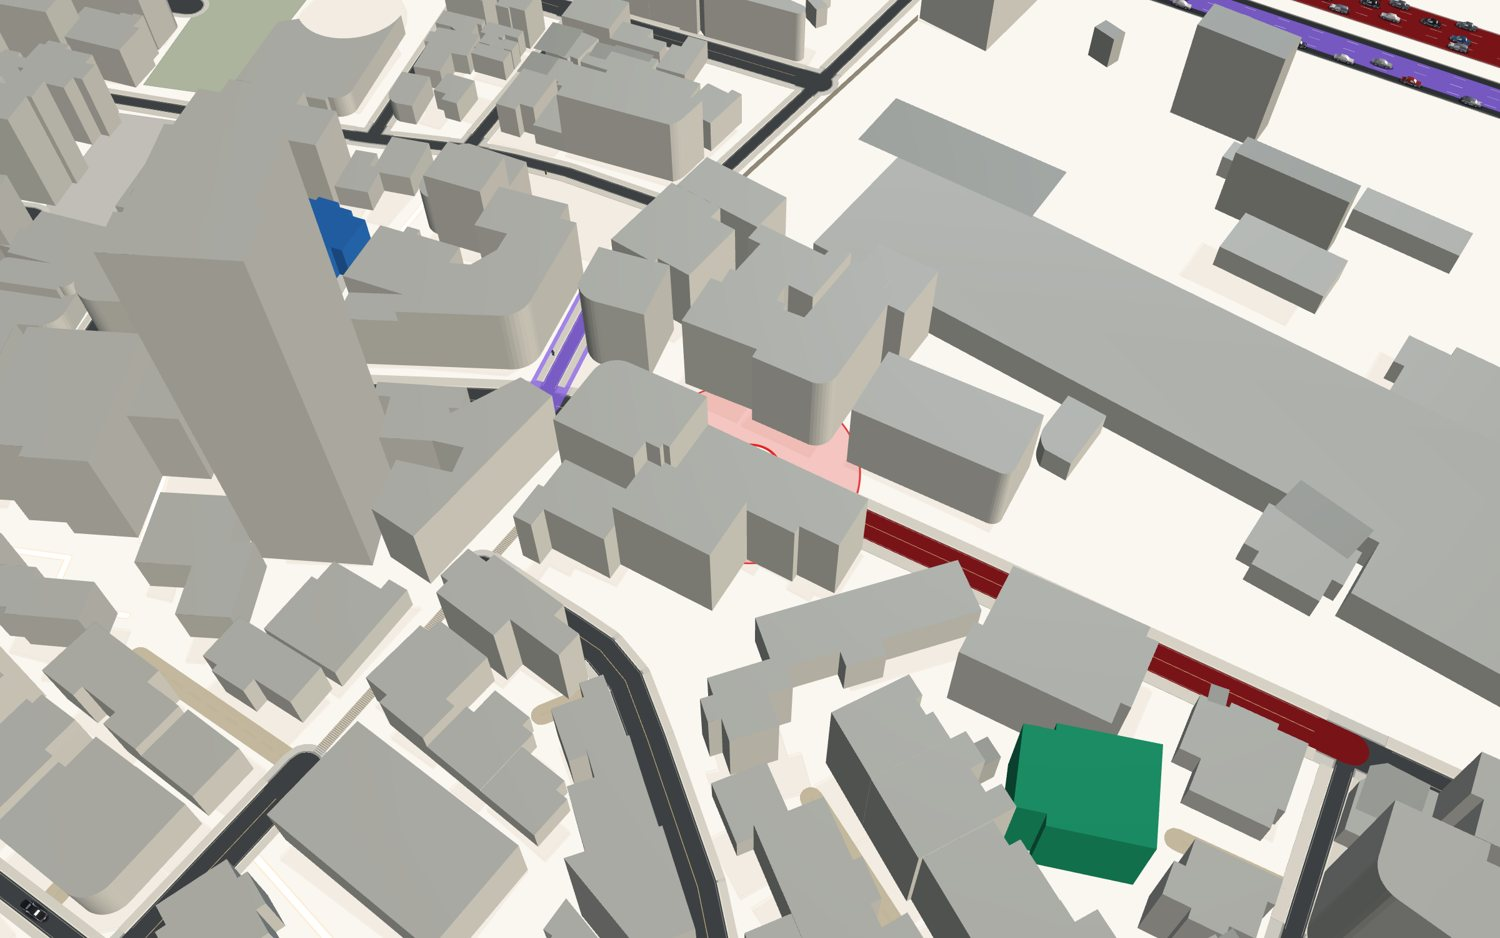
\includegraphics[width=\linewidth]{t_crash}\caption{A crash on Armenia Street (red marker) beside the closed highway.}\end{subfigure}
\caption{Interface and a crash event.}\label{fig:ui}
\end{figure}

\section{Planning streets for pedestrians}
A planner selects one street section (by clicking it or searching by name) and applies a change. SUMO and the pedestrian layer both respond, and the comparison run keeps the original street for reference.

\noindent\begin{minipage}[c]{0.56\linewidth}
\begin{itemize}
\item \textbf{Pedestrianise a section:} motor lanes close in SUMO, cars reroute to parallel streets as in Figure~\ref{fig:detour}, and the pavements stay open (Figure~\ref{fig:carfree}).
\item \textbf{Calm to 30\,km/h (or another limit):} caps the section's SUMO speed. It never raises a lower existing limit.
\item \textbf{Give a lane to the pavements:} a curb-side lane per direction is barred to cars through SUMO lane permissions. The pavement is drawn wider, and the panel reports walking area and modelled walkers per 100\,m$^2$.
\item \textbf{Close a pavement:} that segment's walkers disappear, and the affected occupancy is reported.
\end{itemize}
\end{minipage}\hfill
\begin{minipage}[c]{0.42\linewidth}\centering
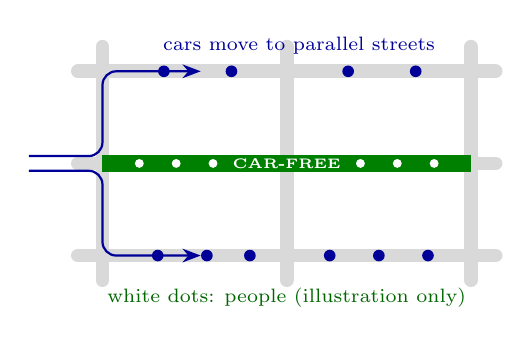
\begin{tikzpicture}[x=0.78cm,y=0.78cm,road/.style={line width=5pt,gray!30,line cap=round}]
  \foreach \y in {0,1.5,3} \draw[road] (0.6,\y) -- (7.4,\y);
  \foreach \x in {1.0,4.0,7.0} \draw[road] (\x,-0.4) -- (\x,3.4);
  \fill[green!50!black] (1.0,1.36) rectangle (7.0,1.64);
  \foreach \x in {1.6,2.2,2.8,5.2,5.8,6.4} \fill[white] (\x,1.5) circle (1.6pt);
  \node[white,font=\tiny\bfseries] at (4.0,1.5) {CAR-FREE};
  \foreach \x in {2.0,3.1,5.0,6.1} \fill[blue!60!black] (\x,3) circle (2.1pt);
  \foreach \x in {1.9,2.7,3.4,4.7,5.5,6.3} \fill[blue!60!black] (\x,0) circle (2.1pt);
  \draw[blue!60!black,thick,-{Stealth},rounded corners=5pt] (-0.2,1.62) -- (1.0,1.62) -- (1.0,3.0) -- (2.6,3.0);
  \draw[blue!60!black,thick,-{Stealth},rounded corners=5pt] (-0.2,1.38) -- (1.0,1.38) -- (1.0,0) -- (2.6,0);
  \node[blue!60!black,font=\scriptsize] at (4.2,3.42) {cars move to parallel streets};
  \node[green!40!black,font=\scriptsize] at (4.0,-0.68) {white dots: people (illustration only)};
\end{tikzpicture}
\captionof{figure}{Pedestrianising a section. (Diagram.)}\label{fig:carfree}
\end{minipage}
\vspace{4pt}

\begin{figure}[H]
\centering
\begin{subfigure}[t]{0.495\linewidth}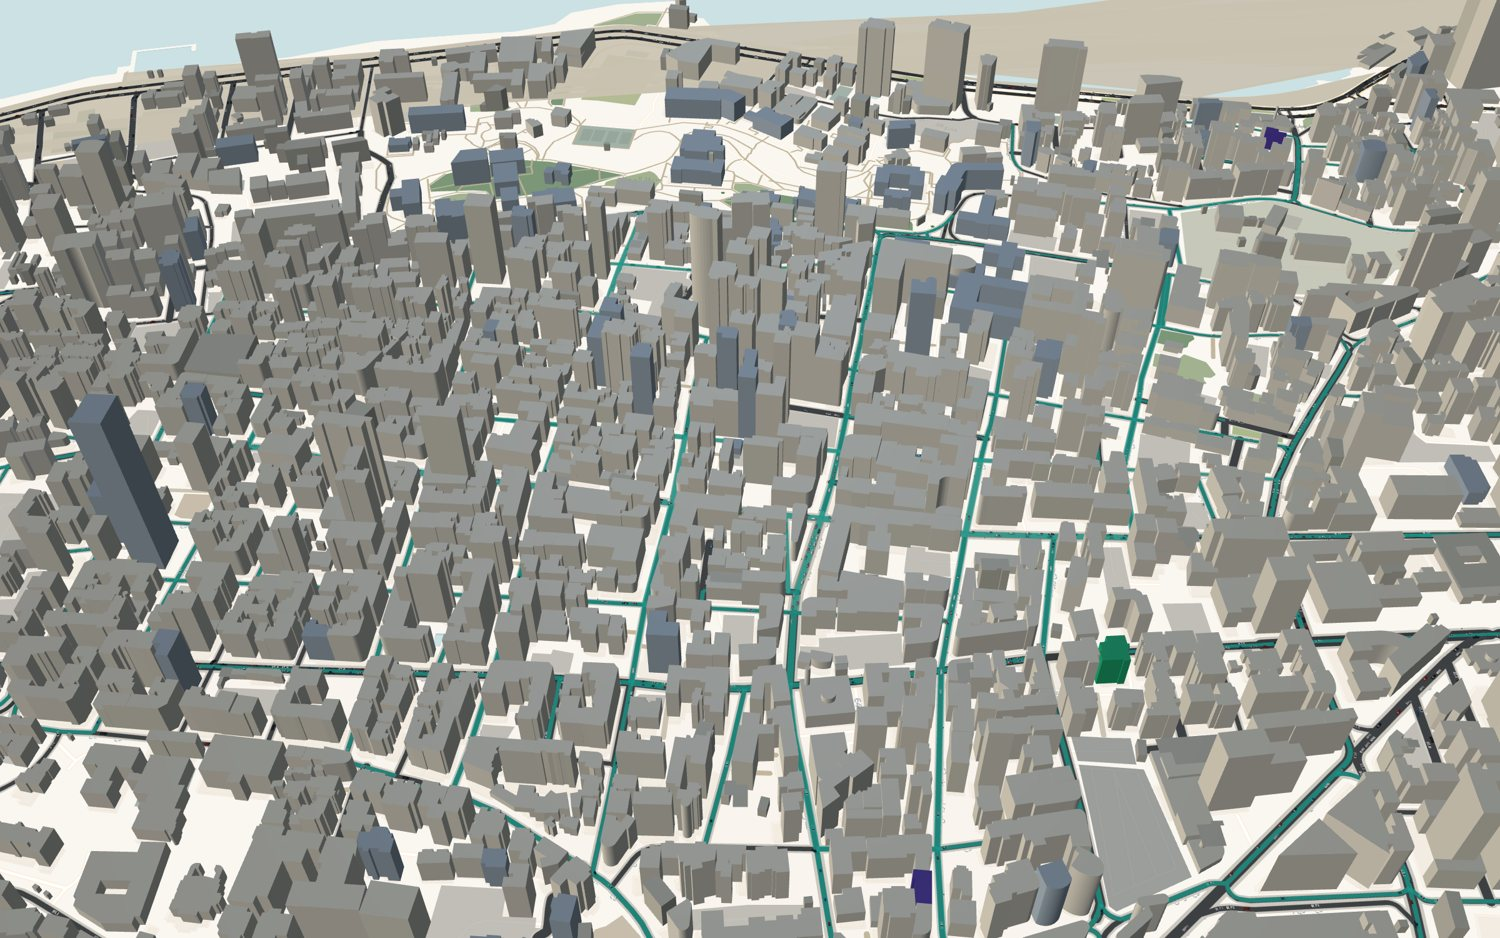
\includegraphics[width=\linewidth]{p_flows}\caption{Modelled PM pedestrian flows around Hamra (green; wider = busier).}\end{subfigure}\hfill
\begin{subfigure}[t]{0.495\linewidth}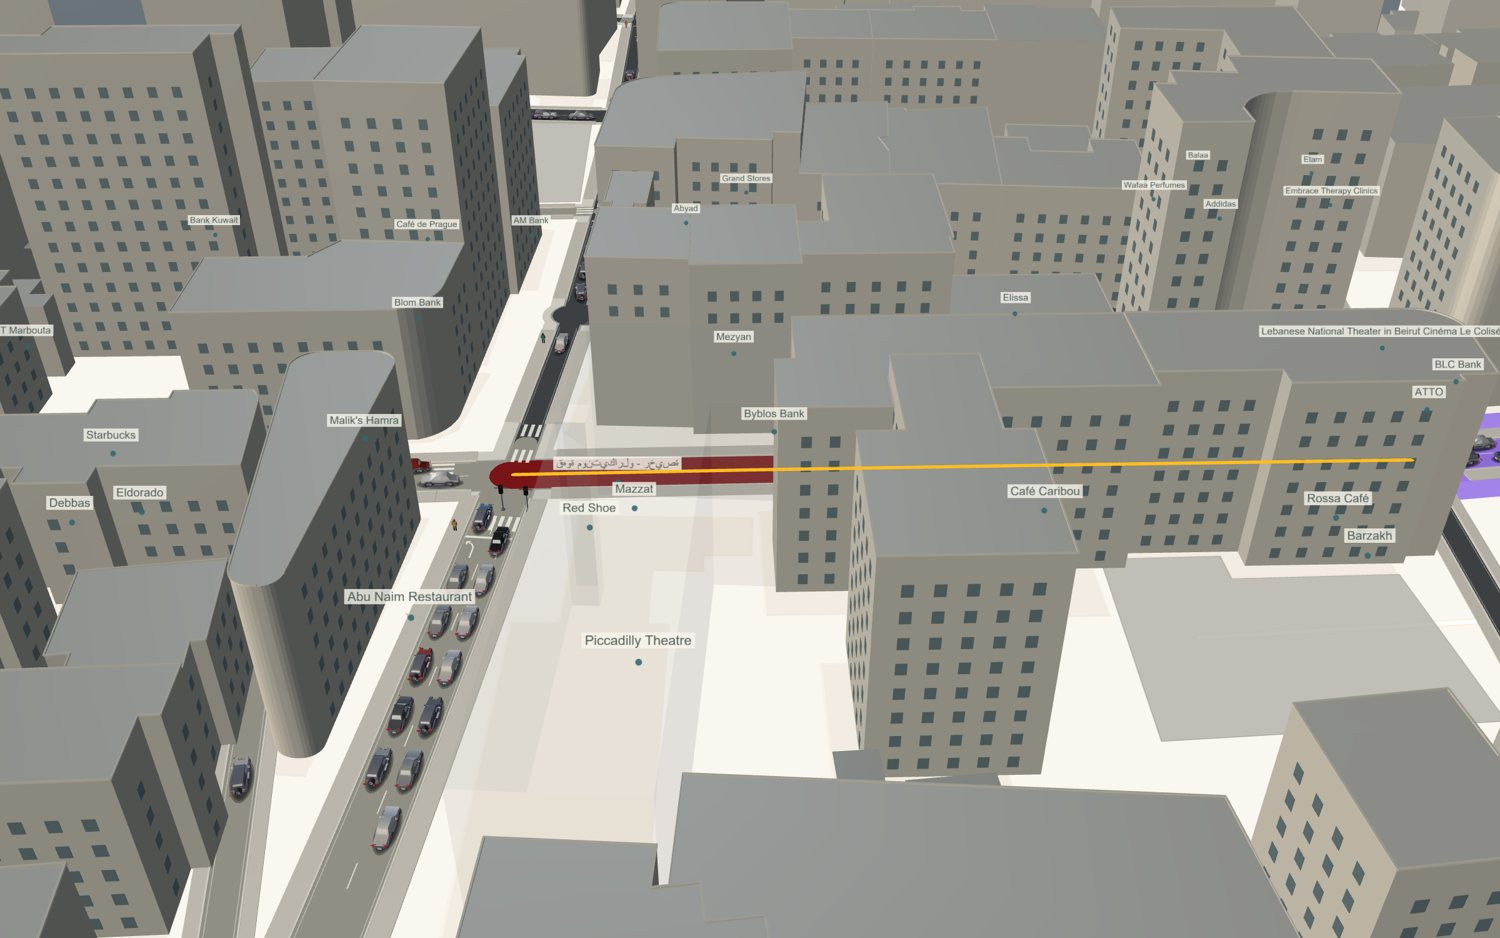
\includegraphics[width=\linewidth]{p_pedestrianised}\caption{A Hamra Street section pedestrianised (red): cars queue and reroute on the cross street.}\end{subfigure}\par\vspace{4pt}
\begin{subfigure}[t]{0.495\linewidth}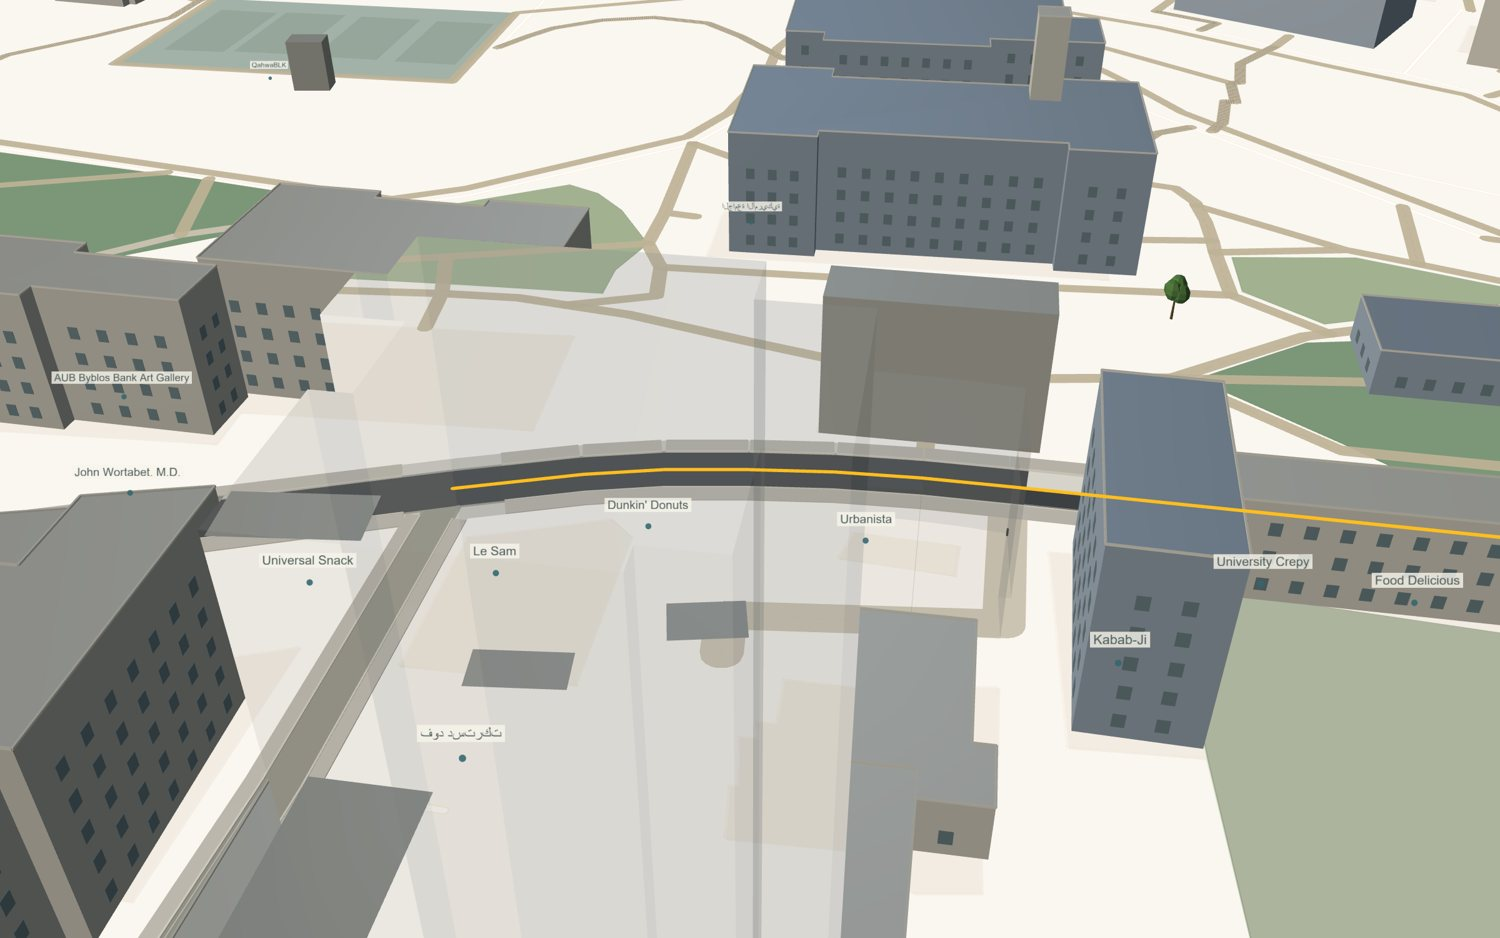
\includegraphics[width=\linewidth]{p_lane}\caption{Bliss Street: the curb lane given to the pavement (orange line).}\end{subfigure}\hfill
\begin{subfigure}[t]{0.495\linewidth}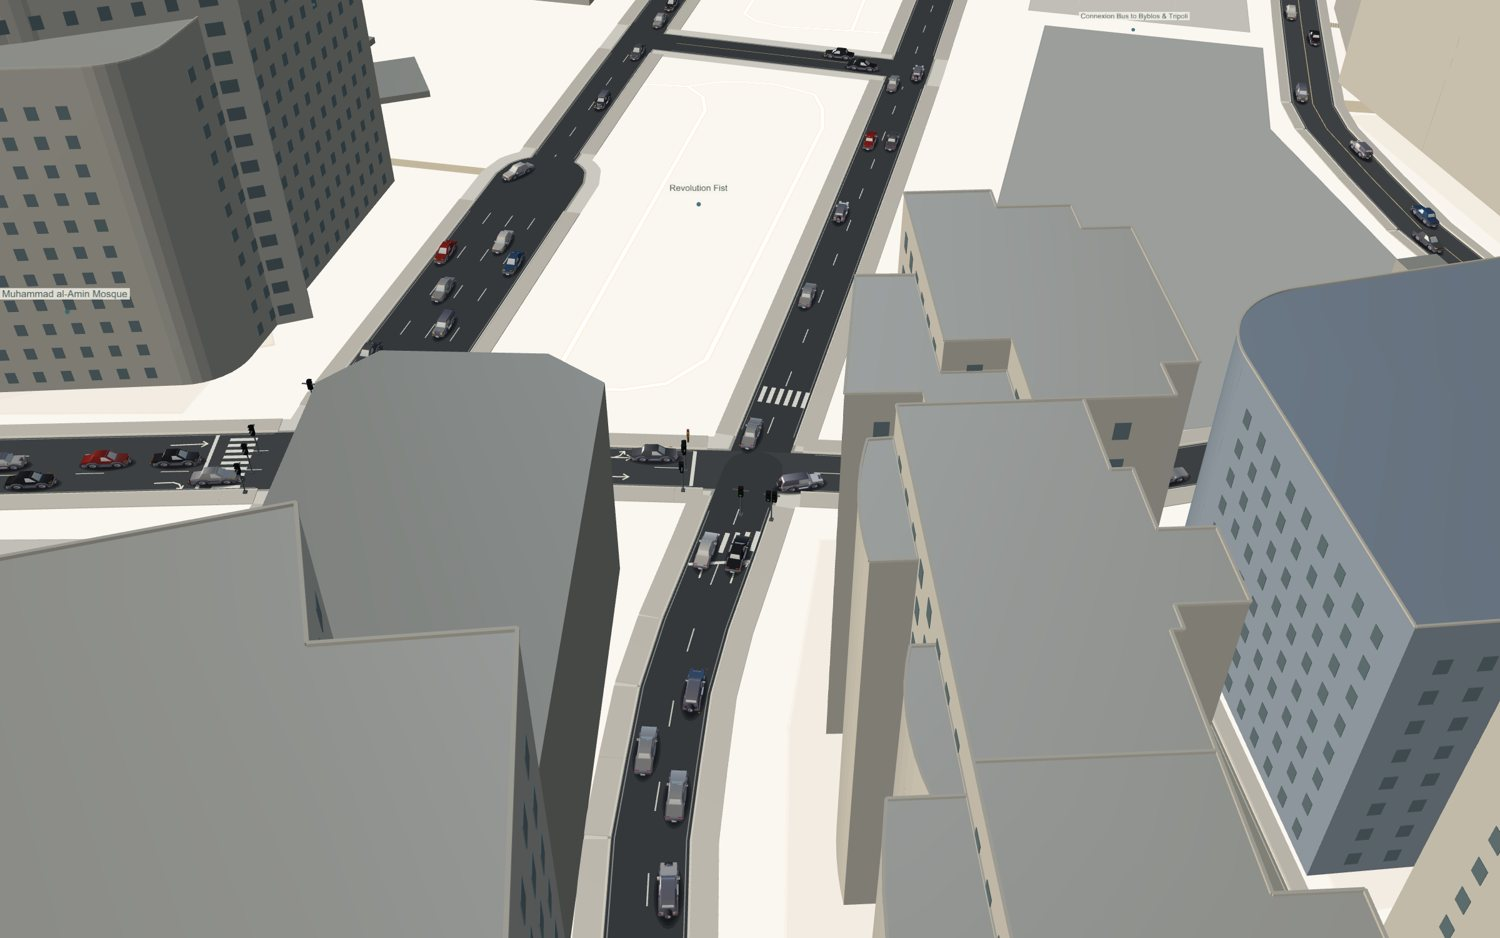
\includegraphics[width=\linewidth]{t_signals}\caption{Simulated signals as 3D poles at a primary junction, 17:00.}\end{subfigure}
\caption{Pedestrian planning tools, and simulated traffic lights at street level.}
\end{figure}

\begin{table}[H]
\centering\small
\begin{tabular}{@{}llrr@{}}
\toprule
Section & Measure & Before & With plan\\
\midrule
Bliss Street (111\,m, one-way, 2 lanes) & Pavement walking space & 535\,m$^2$ & 892\,m$^2$\\
 & Modelled walkers per 100\,m$^2$ & 0.3 & 0.2\\
Hamra Street (119\,m, pedestrianised) & Walking space if the full width is walkable & 572\,m$^2$ & 1,336\,m$^2$\\
 & Modelled walkers per 100\,m$^2$ & 0.8 & 0.3\\
\bottomrule
\end{tabular}
\caption{Indicators reported by the planner for the two changes above.}
\end{table}

\vspace{2pt}{\footnotesize\color{gray}Data credits: Beirut Built Environment Database, Beirut Urban Lab, AUB (ODbL); Beirut 001, Salim al-Kadi and team; OpenStreetMap contributors (ODbL); Overture Maps Foundation; CARTO; Lebanon Traffic Dataset (Tari'ak); CDR BRT ESIA counts; Eclipse SUMO; MIT City Form Lab UNA.}

\end{document}
